\subsection{Library Page (Interface Mockup)}

\begin{figure}[h!]
\centering
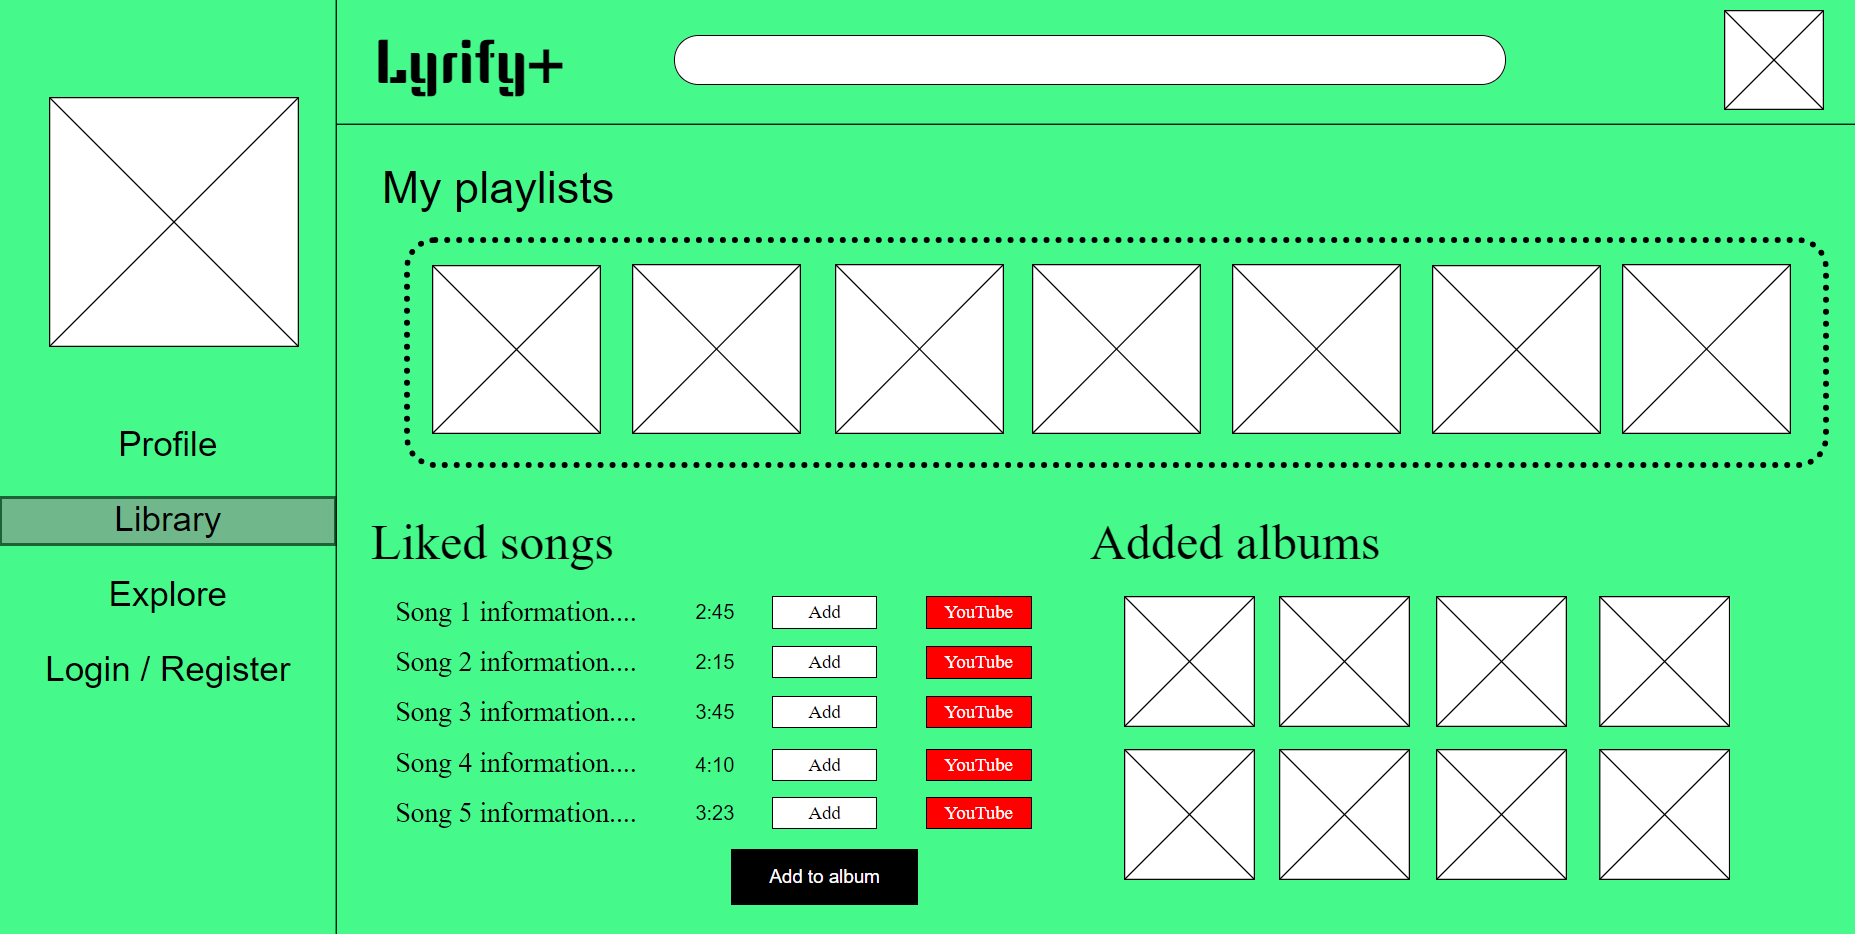
\includegraphics[width=0.9\textwidth]{sections/PLL/LibraryPageMockup.png}
\caption{Library page}
\end{figure}

For this page, we still maintain the design for the side and top panels, with the exception on the darkened ‘Library’ part to show that the user is on the library page. In the center of the page, there will be displayed a row with the user’s playlist that will be empty in the beginning and will grow as the user makes them. On the bottom part, the user will be able to see a small list of the liked songs, showing the names, duration, possibility to add to a playlist and YouTube video button; on the other side a list of the added albums will be displayed too, showing only the albums’ covers. 